\section{Resultados y discusión}

\subsection{Verificación funcional de la Parte A}
El testbench autoverificable se ejecutó en XSim 2025.1 y completó
las 4096 combinaciones binarias de entrada: 256 por cada opcode.
No se detectaron diferencias en Result, Carry, Zero ni en la salida
\texttt{AR\_3V3\_EN}. El último caso se comprobó a los
$40{,}96\,\mu\mathrm{s}$, de acuerdo con los 10 ns asignados a cada
estímulo. El registro terminó con el mensaje
\texttt{PASS: 4096 casos verificados}.

La Figura~\ref{fig:ondas_a_general} muestra el recorrido completo
de la simulación. A esa escala, los cambios de los buses se ven
superpuestos; para interpretar los valores se ampliaron dos casos
de borde en la Figura~\ref{fig:ondas_a_bordes}. Los valores de los
buses se presentan en hexadecimal, con \texttt{SW} organizado como
opcode, $B$ y $A$, de mayor a menor peso.

En el primer caso, a los 2410 ns, \texttt{SW=01f} selecciona
$A=15$, $B=1$ y la suma. Se obtiene \texttt{Result=0},
\texttt{Carry=1} y \texttt{Zero=1}: el resultado matemático es 16,
pero se conservan cuatro bits y el acarreo indica el desbordamiento
sin signo. En el segundo, a los 2570 ns, \texttt{SW=110} selecciona
$A=0$, $B=1$ y la resta. El resultado es \texttt{f} (15),
con \texttt{Carry=1} por préstamo y \texttt{Zero=0}.
En ambos casos la habilitación \texttt{AR\_3V3\_EN} permanece en cero.

\begin{figure*}[!t]
\centering
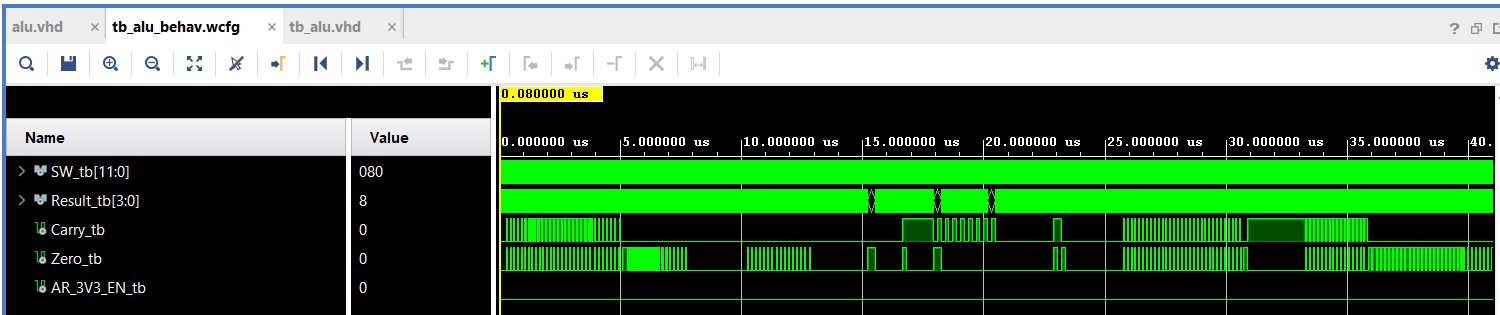
\includegraphics[width=\textwidth]{imagenes/ondas_parte_a_completa.png}
\caption{Simulación funcional completa de la Parte A: 4096 combinaciones de entrada en 40,96 microsegundos.}
\label{fig:ondas_a_general}
\end{figure*}

\begin{figure*}[!t]
\centering
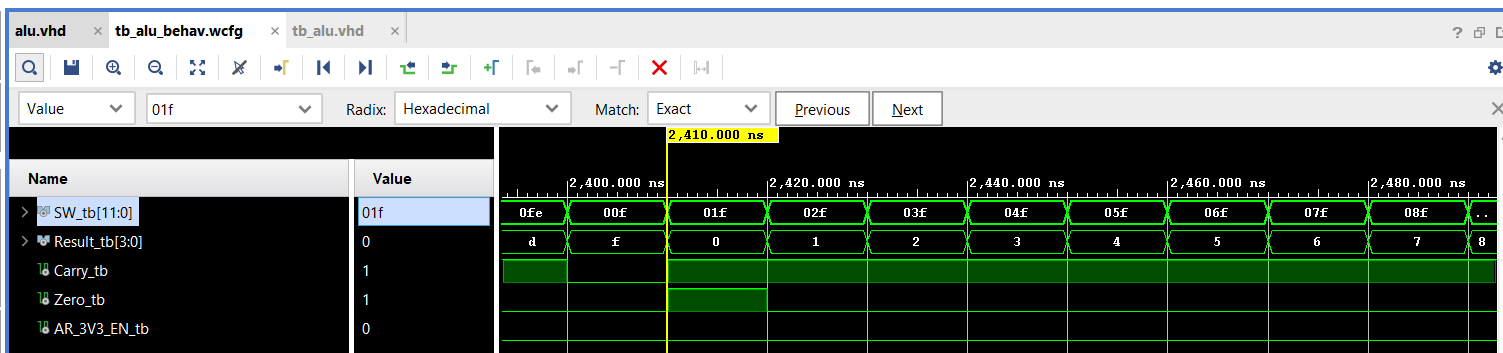
\includegraphics[width=\textwidth]{imagenes/ondas_parte_a_suma_acarreo.png}
\par\medskip
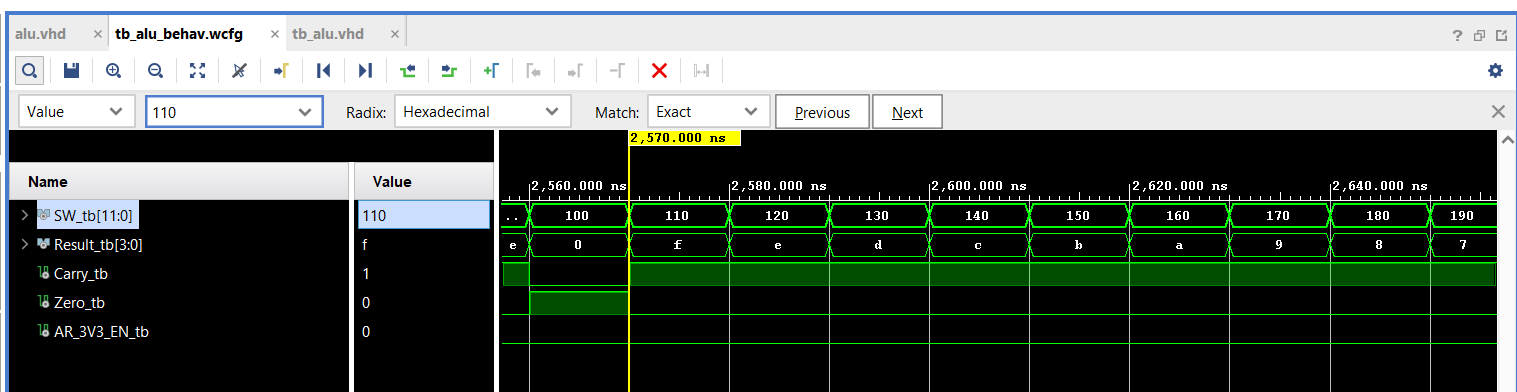
\includegraphics[width=\textwidth]{imagenes/ondas_parte_a_resta_prestamo.png}
\caption{Casos de borde de la Parte A. Arriba: $15+1$, con acarreo y resultado cero. Abajo: $0-1$, con préstamo y resultado de cuatro bits igual a 15.}
\label{fig:ondas_a_bordes}
\end{figure*}

\subsection{Síntesis preliminar de la Parte A}
La síntesis para \texttt{xc7s15ftgb196-1} terminó sin errores ni
advertencias críticas. El reporte de utilización informa 33 Slice
LUTs, seis multiplexores F7 y uno F8; los registros, latches, bloques
de RAM y DSP utilizados son cero. La ausencia de almacenamiento es
coherente con la descripción combinacional prevista. La advertencia
sobre \texttt{AR\_3V3\_EN} conectada a cero corresponde a la
habilitación fija requerida por el shield.

Estos resultados corresponden a simulación funcional y síntesis
sin restricciones XDC. La asignación de pines, la implementación,
la verificación temporal y las pruebas en placa de la Parte A
todavía no se realizaron.
